% Figure: The Security Activation Gap
% Side-by-side comparison: standard IoT deployment vs. methodology-driven.
% Left column: some security controls available but not activated.
% Right column: all controls activated by design through the methodology.
% The gap is shown as a bi-directional annotation between the two.

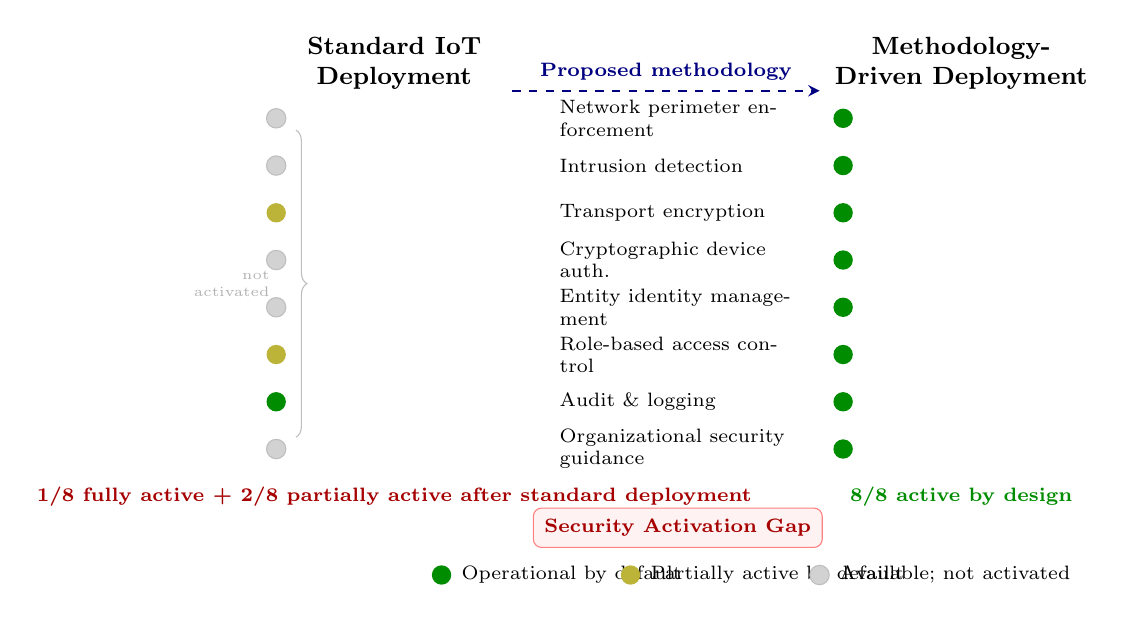
\begin{tikzpicture}[font=\footnotesize]

% ── Styles ──────────────────────────────────────────────────
\tikzset{
  colbox/.style={draw=gray!50, fill=gray!4, rounded corners=5pt,
                 minimum width=3.8cm, inner sep=8pt},
  hdr/.style={font=\bfseries\small, align=center, text width=3.6cm},
  rowlabel/.style={align=left, text width=3.0cm, font=\scriptsize},
  doton/.style={circle, fill=green!55!black, minimum size=7pt, inner sep=0pt},
  dotoff/.style={circle, fill=gray!35, draw=gray!50, minimum size=7pt, inner sep=0pt},
  dotpartial/.style={circle, fill=yellow!70!black, minimum size=7pt, inner sep=0pt},
  gaparrow/.style={<->, very thick, >=stealth, red!65!black},
  methodarrow/.style={->, thick, >=stealth, blue!50!black, dashed}
}

% ── Column x-positions ──────────────────────────────────────
\def\lx{0}      % left column centre
\def\rx{7.2}    % right column centre
\def\dotlx{-1.5}% left dot x
\def\dotrx{5.7} % right dot x
\def\lbllx{-1.1}% left label x
\def\lblrx{6.1} % right label x

% ── Row y-positions (8 controls) ────────────────────────────
\def\rowA{-0.7}
\def\rowB{-1.3}
\def\rowC{-1.9}
\def\rowD{-2.5}
\def\rowE{-3.1}
\def\rowF{-3.7}
\def\rowG{-4.3}
\def\rowH{-4.9}

% ── Column headers ───────────────────────────────────────────
\node[hdr] at (\lx, 0)  {Standard IoT Deployment};
\node[hdr] at (\rx, 0)  {Methodology-Driven Deployment};

% ── Control labels (shared between columns) ──────────────────
\node[rowlabel] at (3.6, \rowA) {Network perimeter enforcement};
\node[rowlabel] at (3.6, \rowB) {Intrusion detection};
\node[rowlabel] at (3.6, \rowC) {Transport encryption};
\node[rowlabel] at (3.6, \rowD) {Cryptographic device auth.};
\node[rowlabel] at (3.6, \rowE) {Entity identity management};
\node[rowlabel] at (3.6, \rowF) {Role-based access control};
\node[rowlabel] at (3.6, \rowG) {Audit \& logging};
\node[rowlabel] at (3.6, \rowH) {Organizational security guidance};

% ── Left column dots (standard: 3/8 active) ─────────────────
\node[dotoff] at (\dotlx, \rowA) {};   % network perimeter: off
\node[dotoff] at (\dotlx, \rowB) {};   % intrusion detect: off
\node[dotpartial]  at (\dotlx, \rowC) {};   % transport encrypt: on (often TLS available)
\node[dotoff] at (\dotlx, \rowD) {};   % device auth: off
\node[dotoff] at (\dotlx, \rowE) {};   % identity mgmt: off
\node[dotpartial]  at (\dotlx, \rowF) {};   % RBAC: partial (typically present but manual)
\node[doton]  at (\dotlx, \rowG) {};   % logging: on (basic)
\node[dotoff] at (\dotlx, \rowH) {};   % org guidance: off

\node[font=\bfseries\scriptsize, text=red!65!black] at (\lx, -5.5)
    {1/8 fully active + 2/8 partially active after standard deployment};

% ── Right column dots (methodology: 8/8 active) ──────────────
\foreach \y in {\rowA, \rowB, \rowC, \rowD, \rowE, \rowF, \rowG, \rowH} {
    \node[doton] at (\dotrx, \y) {};
}

\node[font=\bfseries\scriptsize, text=green!55!black] at (\rx, -5.5)
    {8/8 active by design};

% ── Methodology arrow (left → right) ─────────────────────────
\draw[methodarrow] (1.5, -0.35) -- node[above, font=\scriptsize\bfseries, text=blue!50!black]
    {Proposed methodology} (5.4, -0.35);

% ── Gap braces ───────────────────────────────────────────────
% Left "inactive" brace
\draw[decorate, decoration={brace, amplitude=4pt}, gray!50]
    (\dotlx+0.25, \rowA-0.15) -- (\dotlx+0.25, \rowH+0.15)
    node[midway, left=6pt, font=\tiny, text=gray!60, align=right, text width=1.2cm]
    {not\\ activated};

% Gap label
\node[draw=red!50, fill=red!5, rounded corners=3pt,
      font=\scriptsize\bfseries, text=red!65!black,
      inner sep=4pt] at (3.6, -5.9) {Security Activation Gap};

% Legend
\node[doton,     label={right:\scriptsize Operational by default}]            at (0.6, -6.5) {};
\node[dotpartial, label={right:\scriptsize Partially active by default}]      at (3.0, -6.5) {};
\node[dotoff,    label={right:\scriptsize Available; not activated}]          at (5.4, -6.5) {};

\end{tikzpicture}
